%%%%%%%%%%%%%%%%%%%%%%%%%%%%%%%%%%%%%%%%%%%%%%%%%%%%%%%%%%%%%%%%%%
%%%%%%%%%%%%%%%%%%%%%%%%%%%%%%%%%%%%%%%%%%%%%%%%%%%%%%%%%%%%%%%%%%
%Packages
\documentclass[10pt, a4paper]{article}
\usepackage[top=3cm, bottom=4cm, left=3.5cm, right=3.5cm]{geometry}
\usepackage{amsmath,amsthm,amsfonts,amssymb,amscd, fancyhdr, color, comment, graphicx, environ}
\usepackage{float}
\usepackage{mathrsfs}
\usepackage[math-style=ISO]{unicode-math}
\setmathfont{TeX Gyre Termes Math}
\usepackage{lastpage}
\usepackage[dvipsnames]{xcolor}
\usepackage[framemethod=TikZ]{mdframed}
\usepackage{enumerate}
\usepackage[shortlabels]{enumitem}
\usepackage{fancyhdr}
\usepackage{indentfirst}
\usepackage{listings}
\usepackage{sectsty}
\usepackage{thmtools}
\usepackage{shadethm}
\usepackage{hyperref}
\usepackage{setspace}
\hypersetup{
    colorlinks=true,
    linkcolor=blue,
    filecolor=magenta,      
    urlcolor=blue,
}
\usepackage[makeroom]{cancel}
\usepackage[utf8]{inputenc}
\usepackage[T1]{fontenc}
\usepackage{hyperref}
\hypersetup{colorlinks=true, linkcolor=blue, filecolor=magenta, urlcolor=cyan,}
\urlstyle{same}
\usepackage{amsmath}
\usepackage{amsfonts}
\usepackage{amssymb}
\usepackage[version=4]{mhchem}
\usepackage{stmaryrd}
\usepackage{graphicx}
\usepackage{subcaption}
\usepackage[export]{adjustbox}
\graphicspath{ {./images/} }
\usepackage{listings}
%%%%%%%%%%%%%%%%%%%%%%%%%%%%%%%%%%%%%%%%%%%%%%%%%%%%%%%%%%%%%%%%%%
%%%%%%%%%%%%%%%%%%%%%%%%%%%%%%%%%%%%%%%%%%%%%%%%%%%%%%%%%%%%%%%%%%
%Environment setup
\mdfsetup{skipabove=\topskip,skipbelow=\topskip}
\newrobustcmd\ExampleText{%
An \textit{inhomogeneous linear} differential equation has the form
\begin{align}
L[v ] = f,
\end{align}
where $L$ is a linear differential operator, $v$ is the dependent
variable, and $f$ is a given non−zero function of the independent
variables alone.
}
\mdfdefinestyle{theoremstyle}{%
linecolor=black,linewidth=1pt,%
frametitlerule=true,%
frametitlebackgroundcolor=gray!20,
innertopmargin=\topskip,
}
\mdtheorem[style=theoremstyle]{Problem}{Problem}
\newenvironment{Solution}{\textbf{Solution.}}

\definecolor{codegreen}{rgb}{0,0.6,0}
\definecolor{codegray}{rgb}{0.5,0.5,0.5}
\definecolor{codepurple}{rgb}{0.58,0,0.82}
\definecolor{backcolour}{rgb}{0.95,0.95,0.92}

\lstdefinestyle{mystyle}{
    backgroundcolor=\color{backcolour},   
    commentstyle=\color{codegreen},
    keywordstyle=\color{magenta},
    numberstyle=\tiny\color{codegray},
    stringstyle=\color{codepurple},
    basicstyle=\ttfamily\footnotesize,
    breakatwhitespace=false,         
    breaklines=true,                 
    captionpos=b,                    
    keepspaces=true,                 
    numbers=left,                    
    numbersep=5pt,                  
    showspaces=false,                
    showstringspaces=false,
    showtabs=false,                  
    tabsize=2
}

\lstset{style=mystyle}
%%%%%%%%%%%%%%%%%%%%%%%%%%%%%%%%%%%%%%%%%%%%%%%%%%%%%%%%%%%%%%%%%%
%%%%%%%%%%%%%%%%%%%%%%%%%%%%%%%%%%%%%%%%%%%%%%%%%%%%%%%%%%%%%%%%%%
%Fill in the appropriate information below
\newcommand{\norm}[1]{\left\lVert#1\right\rVert}     
\newcommand\course{CS5785}                            % <-- course name   
\newcommand\hwnumber{3}                                 % <-- homework number
\newcommand\Information{Arystan Tatishev, Maanas Peri}                        % <-- personal information
%%%%%%%%%%%%%%%%%%%%%%%%%%%%%%%%%%%%%%%%%%%%%%%%%%%%%%%%%%%%%%%%%%
%%%%%%%%%%%%%%%%%%%%%%%%%%%%%%%%%%%%%%%%%%%%%%%%%%%%%%%%%%%%%%%%%%
%Page setup
\pagestyle{fancy}
\headheight 35pt
\lhead{\today}
\rhead{
\includegraphics[width=2.5cm]{logo-ct.png}}
\lfoot{}
\pagenumbering{arabic}
\cfoot{\small\thepage}
\rfoot{}
\headsep 1.2em
\renewcommand{\baselinestretch}{1.25}
%%%%%%%%%%%%%%%%%%%%%%%%%%%%%%%%%%%%%%%%%%%%%%%%%%%%%%%%%%%%%%%%%%
%%%%%%%%%%%%%%%%%%%%%%%%%%%%%%%%%%%%%%%%%%%%%%%%%%%%%%%%%%%%%%%%%%
%Add new commands here
\renewcommand{\labelenumi}{\alph{enumi})}
\newcommand{\Z}{\mathbb Z}
\newcommand{\R}{\mathbb R}
\newcommand{\Q}{\mathbb Q}
\newcommand{\NN}{\mathbb N}
\newcommand{\PP}{\mathbb P}
\DeclareMathOperator{\Mod}{Mod} 
\renewcommand\lstlistingname{Algorithm}
\renewcommand\lstlistlistingname{Algorithms}
\def\lstlistingautorefname{Alg.}
\newtheorem*{theorem}{Theorem}
\newtheorem*{lemma}{Lemma}
\newtheorem{case}{Case}
\newcommand{\assign}{:=}
\newcommand{\infixiff}{\text{ iff }}
\newcommand{\nobracket}{}
\newcommand{\backassign}{=:}
\newcommand{\tmmathbf}[1]{\ensuremath{\boldsymbol{#1}}}
\newcommand{\tmop}[1]{\ensuremath{\operatorname{#1}}}
\newcommand{\tmtextbf}[1]{\text{{\bfseries{#1}}}}
\newcommand{\tmtextit}[1]{\text{{\itshape{#1}}}}

\newenvironment{itemizedot}{\begin{itemize} \renewcommand{\labelitemi}{$\bullet$}\renewcommand{\labelitemii}{$\bullet$}\renewcommand{\labelitemiii}{$\bullet$}\renewcommand{\labelitemiv}{$\bullet$}}{\end{itemize}}
\catcode`\<=\active \def<{
\fontencoding{T1}\selectfont\symbol{60}\fontencoding{\encodingdefault}}
\catcode`\>=\active \def>{
\fontencoding{T1}\selectfont\symbol{62}\fontencoding{\encodingdefault}}
\catcode`\<=\active \def<{
\fontencoding{T1}\selectfont\symbol{60}\fontencoding{\encodingdefault}}

%%%%%%%%%%%%%%%%%%%%%%%%%%%%%%%%%%%%%%%%%%%%%%%%%%%%%%%%%%%%%%%%%%
%%%%%%%%%%%%%%%%%%%%%%%%%%%%%%%%%%%%%%%%%%%%%%%%%%%%%%%%%%%%%%%%%%
%Begin now!

\begin{document}
\section{SHORT QUESTIONS (30PT)}
\begin{enumerate}[label=(\alph*)]
    \item (2pt) When we run K-Means on the same dataset with different starting conditions, we can get different clusterings. True or False?

    \item[Explanation:] True, because K-Means can fall into local minimas

    \item (2pt) Linear Discriminant Analysis assumes that the class conditioned densities are Gaussian with the same covariance matrix. True or False?

    \item[Explanation:] True, When the covariances in GDA are equal, we have an algorithm called Linear Discriminant Analysis or LDA.

    \item (2pt) Kernelized SVM and Kernelized Ridge Regression are examples of non-parametric models. True or False?

    \item[Explanation:] False, KSVM and KRR are parametric models

    \item (2pt) KNN is an example of supervised learning method. True or False?

    \item[Explanation:] True, KNN is a supervised learning method

    \item (2pt) Suppose we are running the SVM algorithm on a binary classification task that has labels +1 and -1 . Let $f$ be the score function that maps inputs $x$ to real numbers. Using the hinge loss, for a data point $(x, y)$ that has label value $y=+1$, all predictions $f(x) \geq 1$ will incur the same loss. True or False?.

    \item[Explanation:] True, SVM does not penalize correct predictions

    \item (2pt) List three methods commonly used for handling overfitting:

    \item[Explanation:] Use a simpler model family, collect more training data or modify the training process to penalize overly complex models

    \item (2pt) Given a design matrix $X$, the normal equations $\left(X^{\top} X\right)^{-1} X^{\top} y$ always involve an invertible matrix $\left(X^{\top} X\right)$. True or False?

    \item[Explanation:] False, we only assume the matrix is invertible

    \item (2pt) The kernel trick can only be used to efficiently compute the dot product between finite-dimensional features $\phi(x)$. True or False?

    \item[Explanation:] False, We can efficiently use any features $\phi(x)$ up to infinite dimensions i.e. Taylor Series

    \item (2pt) A Kaggle competition typically has two different test sets. One set is used to score the public leaderboard during the competition. The other set is used to create a private leaderboard after the competition ends. One team repeatedly submits their method on the public set, making small changes each time until they achieve first place on the public leaderboard. When the competition ends, teams are re-scored on the private set. The team finds they have dropped to $102^{\text {nd }}$ place. What happened? Please describe.

    \item[Explanation:] The team has overfitted their model that performs extremely well on a public set. However, since their data was trained exclusively on a public set, the private set did not fit their model well, rather than the opposite.

    For each of the listed descriptions below, choose whether the experimental set up is ok or problematic. If you think it is problematic, briefly state what the problems are:

    \item (4pt) A team is building a 10-class digit classifier. They're trying out a new method of cross-validation. Instead of choosing the folds randomly, they constrain each fold to contain only a single digit class. Ok or Problematic?

    \item[Explanation:] Problematic, By constraining each fold to contain only a single digit class, the training set for each fold will lack 9 out of the 10 classes

    \item (4pt) A team is using $k$-nearest neighbor to classify birds. They use 10 -fold cross validation to pick the $k$ that maximizes the average validation accuracy. Ok or Problematic?

    \item[Explanation:] Ok, Using \(k\)-fold cross-validation to pick the \(k\) that maximizes the average validation accuracy is a standard and widely accepted approach for hyperparameter tuning.

    \item (4pt) Suppose an intern at Google is trying to build a better spam classifier. They believe their model is good because every spam message in their test set was caught and correctly classified as spam. Ok or Problematic?

    \item[Explanation:] Problematic, if their model catches every single spam message then they are likely overfitting their model to cater to the test set
\end{enumerate}

\section{Probability and MLE [20 POINTS]:}
Let $x$ be the time interval (in hour) between two messages on CS5785 Slack team. Assume that $x$ has the following probability density function:

$$
p(x ; \theta)= \begin{cases}\theta^{-1} e^{-x / \theta}, & \text { if } x \geq 0 \\ 0, & \text { otherwise }\end{cases}
$$

You check the Slack team several times and get 4 independent observations of $x: x_{1}=0.2, x_{2}=0.3, x_{3}=0.5, x_{4}=1$.

\begin{enumerate}[label = (\alph*)]
    \item (10pt) What is the log-likelihood of your observations given $\theta=1$ ?

    \item[Answer] Plug in your observations \( x_1=0.2, x_2=0.3, x_3=0.5, x_4=1 \) and \( \theta=1 \) to get the likelihood:
    
    \[ L(1; 0.2, 0.3, 0.5, 1) = p(0.2;1) \times p(0.3;1) \times p(0.5;1) \times p(1;1) \]
    \[ = e^{-0.2} \times e^{-0.3} \times e^{-0.5} \times e^{-1} \]
    
    Take the natural log to get the log-likelihood:
    
    \[ l(1; 0.2, 0.3, 0.5, 1) = \ln(e^{-0.2} \times e^{-0.3} \times e^{-0.5} \times e^{-1}) \]
    \[ = (-0.2) + (-0.3) + (-0.5) + (-1) \]
    \[ = -2 \]
    
    So, the log-likelihood of the observations given \( \theta=1 \) is -2.

    \item (10pt) What value of $\theta$ maximizes the likelihood? Provide justification via mathematical deduction.

    \item[Answer] To find the value of \( \theta \) that maximizes the likelihood, we need to take the derivative of the log-likelihood with respect to \( \theta \), set it to zero, and solve for \( \theta \). This will give us the maximum likelihood estimate (MLE) of \( \theta \).

    The log-likelihood is:
    
    \[ l(\theta) = \sum_{i=1}^{4} \ln(p(x_i ; \theta)) \]
    \[ = \sum_{i=1}^{4} \left( -\ln(\theta) - \frac{x_i}{\theta} \right) \]
    \[ = -4\ln(\theta) - \frac{1}{\theta} \sum_{i=1}^{4} x_i \]
    
    Differentiating with respect to \( \theta \):
    
    \[ \frac{\partial l(\theta)}{\partial \theta} = -\frac{4}{\theta} + \frac{1}{\theta^2} \sum_{i=1}^{4} x_i \]
    
    Setting the derivative to zero to find the extrema:
    
    \[ -\frac{4}{\theta} + \frac{1}{\theta^2} \sum_{i=1}^{4} x_i = 0 \]
    
    \[ -4\theta + \sum_{i=1}^{4} x_i = 0 \]
    
    \[ \implies \theta = \frac{\sum_{i=1}^{4} x_i}{4} \]
    
    \[ \theta = \frac{0.2 + 0.3 + 0.5 + 1}{4} = \frac{2}{4} = 0.5 \]
\end{enumerate}

\section{DECISION BOUNDARIES (15PT)}
\begin{enumerate}[label = \alph*]
    \item (2pt each; 10 total) Here are several binary classification algorithms. Match the decision boundary with the classification method; you should write down the letter corresponding to the plot next to each classifier name. Each plot corresponds to one algorithm on the left; select the best match.

    \begin{itemize}
        \begin{figure}[H]
            \centering
            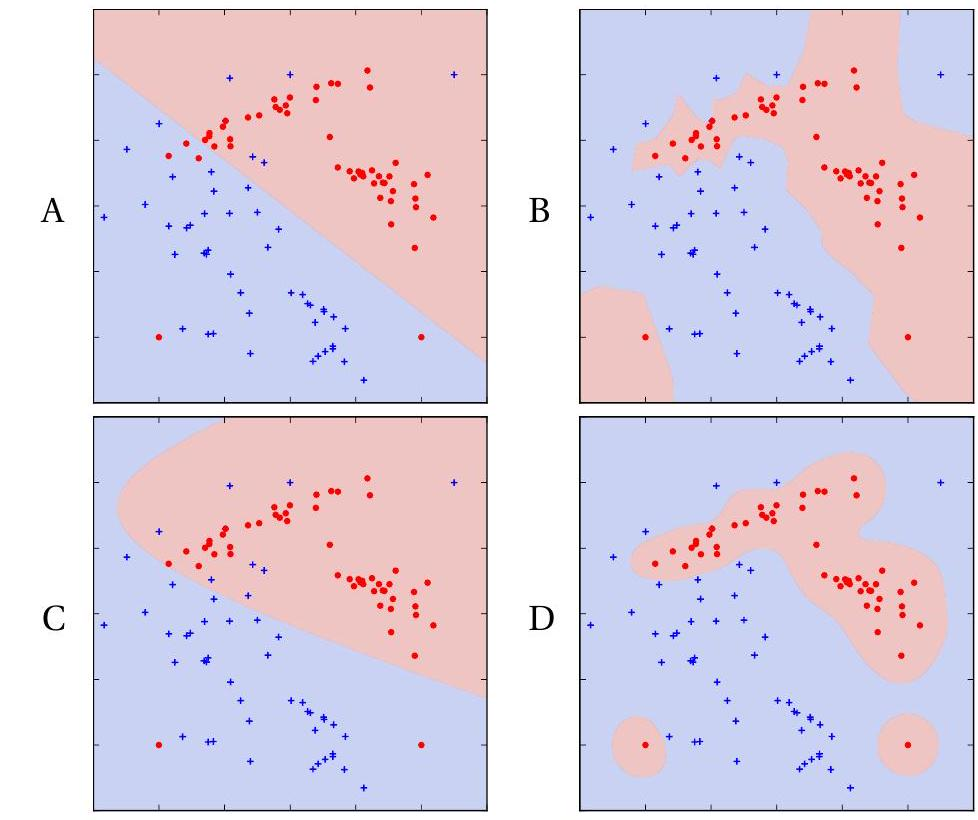
\includegraphics[width=0.5\linewidth]{Prelim/2023_10_21_60a0f388d4d807b89e95g-05.jpg}
            \caption{Enter Caption}
            \label{fig:enter-label}
        \end{figure}
        
        \item $k$-NN, for $k=1$ :

        \item[Answer:] B, This classifier would have boundaries that are extremely flexible and sensitive to individual data points, effectively "hugging" the data closely.

        \item SVM, polynomial kernel kernel:

        \item[Answer:] C, The SVM with a polynomial kernel would produce curved decision boundaries, but they would typically be smoother and more systematic than the extremely flexible boundaries of a 1-NN classifier.

        \item Linear discriminant analysis:

        \item[Answer:] A, LDA tries to find a linear combination of features that characterizes or separates two or more classes. Therefore, the decision boundary is linear.

        \item SVM, radial basis function kernel:

        \item[Answer:] D, The RBF kernel in SVM can create non-linear decision boundaries and is capable of forming more complex shapes, like circles or ellipses around data clusters.
    \end{itemize}

    \item (5pt) Which classifier has the most similar decision boundary to an SVM with the primal formulation?

    \item[Answer] The SVM with the primal formulation refers to an SVM that uses a linear kernel. The primal problem for SVMs represents a linear decision boundary in the input space.

    Given this, the classifier with the most similar decision boundary to an SVM with the primal formulation is the one with a linear decision boundary.
    
    From the provided plots, Plot A shows a clear linear boundary. Therefore, the classifier that has the most similar decision boundary to an SVM with the primal formulation is the one represented by Plot A, which is the Linear discriminant analysis (LDA).
\end{enumerate}

\section{Principal Component Analysis (15 PT)}
Given four 2D data points $(-2,-2),(2,2),(-1,1),(1,-1)$, and we want to perform Principal Component Analysis (PCA) to project the data points into compact 1D space.

\begin{enumerate}[label = \arabic*.]
  \item (5pt) Find the first principal component of the four $2 \mathrm{D}$ data points. This is a $2 \mathrm{D}$ eigenvector with the largest eigenvalue in eigendecomposition. \textbf{Hint:} \textit{You can first plot the data points and think about the alignment of data points visually. It's possible to obtain the principal components without manually performing eigendecomposition so you should not need to do that. Also, if a vector is the first principal component, its negation is also the first principal component, so feel free to provide just one of them.}

  \item[Answer:] Vector of y=x. [1, 1]

  \item (5pt) The objective of PCA is to choose a projection direction that maximizes the variance of projected data points. What is the variance of the projected 1D data points?

  \item[Answer:] Compute the variance:
\[ \text{Variance} = \frac{1}{N} \sum_{i=1}^{N} (x_i - \mu)^2 \]
Where \(x_i\) are the data points and \(\mu\) is the mean of the data points.

For our data, the mean, \(\mu\), is 0 (since the mean of the projected coordinates is 0).

Thus, the variance is:
\[ \text{Variance} = \frac{1}{4} [(-2\sqrt{2})^2 + (2\sqrt{2})^2 + 0^2 + 0^2] \]
\[ \text{Variance} = \frac{1}{4} [8 + 8] = 4 \]

Therefore, the variance of the projected 1D data points is \(4\).

  \item (5pt) An alternative objective of PCA is minimizing the reconstruction error. What is the reconstruction error? \textbf{Hint:} \textit{Recall that given $N$ data points $x^{(i)} \in \mathbb{R}^{2}$ (for $i=1, \ldots, N$ ) and the orthonormal projection matrix $W \in \mathbb{R}^{2 \times 1}$, the reconstruction error is given by $J(W)=\sum_{i=1}^{N}\left\|x^{(i)}-W W^{T} x^{(i)}\right\|_{2}^{2}$.}

  \item[Answer:] The reconstruction error for points 1 and 2 is 0 since they lie on the vector line. For points 3 and 4, it is 2 since the squares of the distance between the vector and the point is 2. Thus the total is $0 + 0 + 2 + 2 = 4$

\end{enumerate}

\section{NAÏVE BAYES WITH BAG-OF-WORDS (20PT)}
We are building a twitter robot that can tell the difference between tweets about sports versus academic tweets about machine learning conferences. Our students have scoured twitter, collecting a dataset as follows. Each tweet is labeled with either sports or machine learning.

\begin{center}
\begin{tabular}{l|l}
\textit{Sports} & \textit{Machine learning} \\
\hline
\begin{tabular}{l}
Red Sox \textbf{win} big last week, \textbf{score} 36-35 against \\
Yankees \\
\end{tabular} & \begin{tabular}{l}
\textbf{Deep Learning} models using rectified lin- \\
ear \textbf{loss} functions \textbf{score} better than hand- \\
selected baselines in latest competition! \\
\end{tabular} \\
\hline
\begin{tabular}{l}
\textbf{Learning} their place on the new food chain, \\
patriots suffer another \textbf{deep loss} \\
\end{tabular} & \begin{tabular}{l}
More \textbf{deep} model magic! Yann LeCun for the \\
\textbf{win}! \\
\end{tabular} \\
\hline
\begin{tabular}{l}
Giants \textbf{score} 42 points for the \textbf{win}, averting \\
another \textbf{loss} in the semifinals \\
\end{tabular} & \begin{tabular}{l}
Reinforcement \textbf{learning} is the wave of the fu- \\
ture \\
\end{tabular} \\
\hline
\end{tabular} \\
\end{center}

\begin{enumerate}[label = \alph*]
    \item (10pt) Convert the above tweets into a bag of words representation, a binary vector with five elements. Calculate $P$ (word $i$ present|class), for each of the important bolded words: \textbf{Win}, \textbf{Loss}, \textbf{Learning}, \textbf{Score}, \textbf{Deep}.

    \item[Answer:] 

    \item (10pt) Consider the following tweet: 

    Latest ResNet is crushing the ImageNet competition, with lower \textbf{loss} value than other models! Another big \textbf{win} for \textbf{deep learning}!

    Let $x$ be its bag-of-words vector. What probability $P\left(\operatorname{class}_{\mathrm{ML}} \mid x\right)$ and $P\left(\operatorname{class}_{\text {sparts }} \mid x\right)$ would a Naive Bayes classifier assign to this tweet? What label would it assign?

    \item[Answer:] 
\end{enumerate}

\end{document}